\documentclass[solutions]{esg8022pset} 
\usepackage{amsmath}
\usepackage{amssymb}
\usepackage{enumerate}
\usepackage{graphicx}
\usepackage{hyperref}
\usepackage{mathtools}
\usepackage[per-mode=symbol]{siunitx} %If this line is giving you trouble, try replacing per-mode with per
%use inter-unit-separator={}\cdot{} ?
\providecommand{\uvec}[1]{{\hat{\bf{#1}}}}
\usepackage{pgf,tikz}
\usetikzlibrary{arrows}
\usepackage{wasysym}
\usepackage{subfig}
\makeatletter
\newcommand{\interitemtext}[1]{%
  \begin{list}{}
   {\itemindent=0mm\labelsep=0mm
   \labelwidth=0mm\leftmargin=0mm
   \addtolength{\leftmargin}{-\@totalleftmargin}}
    \item #1
  \end{list}
}
\makeatother
\renewcommand{\d}{\,d}
\providecommand{\norm}[1]{\lVert#1\rVert}

\newcommand{\Kgrad}{\left(\hat{x} \frac{\partial}{\partial x} + \hat{y} \frac{\partial}{\partial y} + \hat{z} \frac{\partial}{\partial z}\right)}
\newcommand{\Kdiv}[6]{{#4}\left(\frac{\partial {#1}}{\partial x} {#5} \frac{\partial {#2}}{\partial y} {#6}\frac{\partial #3}{\partial z} \right)}
\newcommand{\KKdiv}[6]{{#4}\left(\frac{\partial}{\partial x}{#1} {#5} \frac{\partial}{\partial y}{#2} {#6}\frac{\partial}{\partial z}{#3} \right)}
\newcommand{\dx}{\frac{\partial}{\partial x}}
\newcommand{\dy}{\frac{\partial}{\partial y}}
\newcommand{\dz}{\frac{\partial}{\partial z}}
\newcommand{\dtheta}{\frac{\partial}{\partial \theta}}
\newcommand{\dr}{\frac{\partial}{\partial r}}

\AtBeginDocument{%
  % Appologies to any future editor on the inconsistencies in TeX code and the unnecessary braces.  I'm aggregating previously typeset problems, and didn't think it worth my time to improve the quality of TeX code in ways that won't make any difference to the typeset material. -Jason Gross (jgross@mit.edu)
}%
\classname{Physics 8.022} \semester{Spring 2011} 
\problemsetnumber{8}
\date{\today }
\duedate{Sunday, April 3rd at 9 pm}
\readingassignment{}
\problemsettitle{Amp\`{e}re's law, Biot-Savart law}
\begin{document}
\section{Problem \thesection: Long flat conductor}
\subsection{Problem}
A long flat conductor of width $a$ carries a sheet of current $i$ (see figure \ref{fig:flat}). You are asked to find the magnetic  field (direction and magnitude) near the center of
its flat side and and very close to the surface, such that the distance R from the sheet is $R<<a$.

      \begin{figure}[ht]
       \begin{center}
        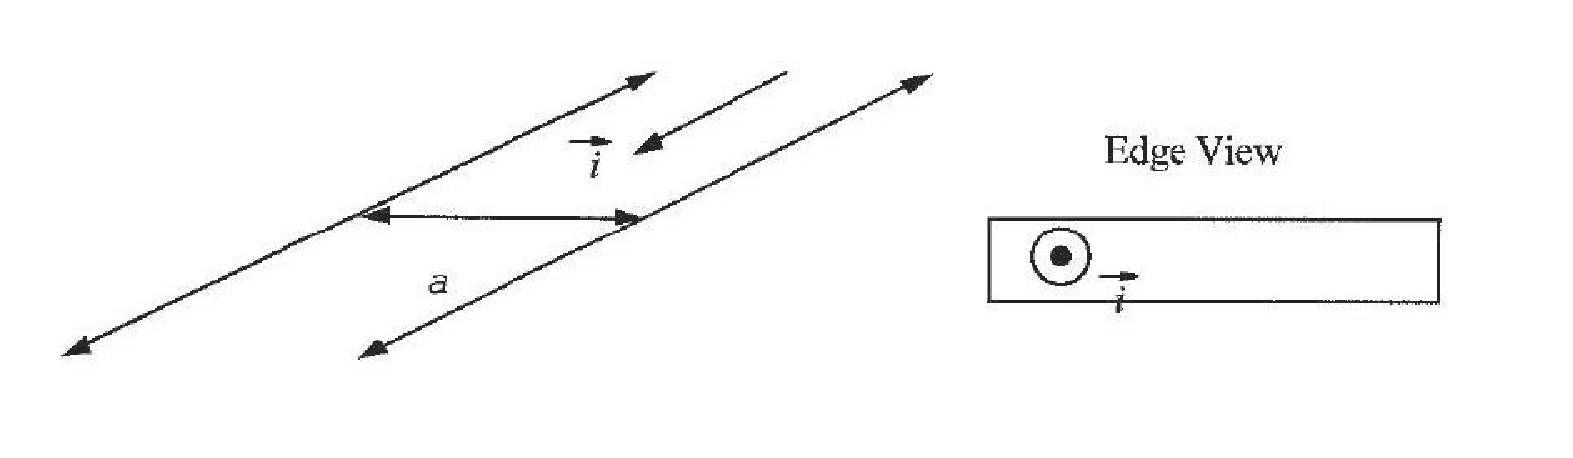
\epsfig{file = flat_conductor.eps, width = 10cm}
        \caption{Flat conductor}
        \end{center}
        \label{fig:flat}
      \end{figure}

\subsection{Solution}

      \begin{figure}[ht]
        \centering
        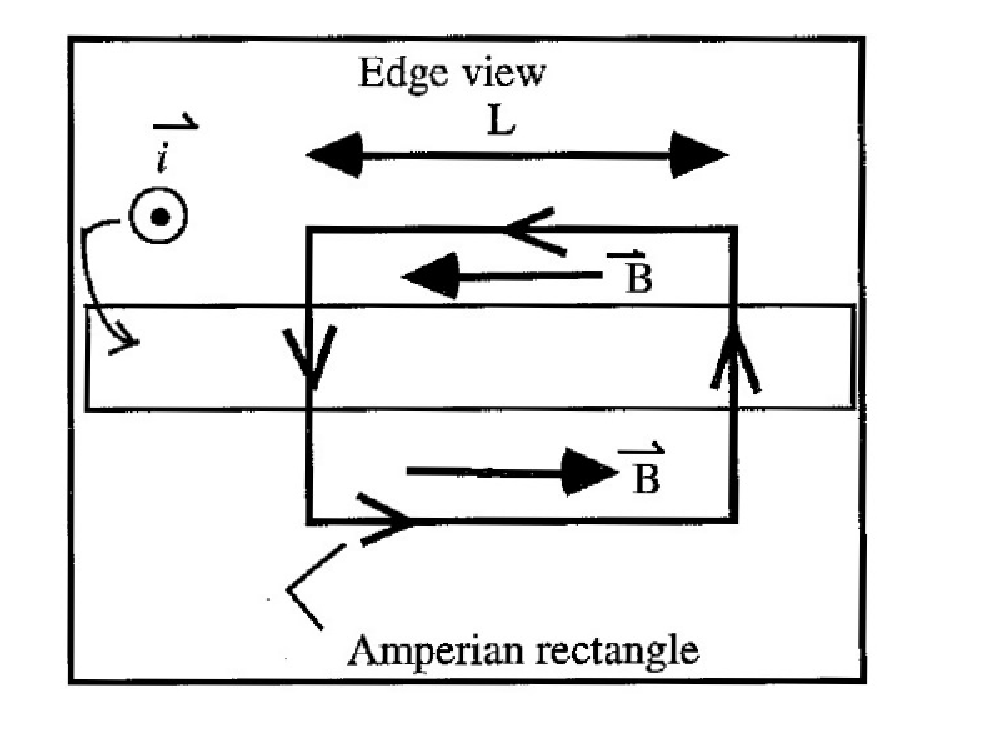
\epsfig{file = flat_conductor_sol}.eps, width = 10cm}
        \label{fig:flatsol}
      \end{figure}

As shown in the figure, above the conductor, \vec{B} points to the left, below the con-
ductor,  \vec{B}  points to the right (the current is pointing out of the paper).
Choose an amperian path shown in the plot, since the distance R is much smaller
than $a$, we have:
\begin{equation}
2B � L = \frac{4 \pi}{c} I_{enc} = \frac{4 \pi}{c} \frac{L i}{a}
\end{equation}
Hence $B=\frac{2 \pi i}{a c}$.
\end{document}
